\begin{figure}[H]
  \centering
  

\tikzset{every picture/.style={line width=0.75pt}} %set default line width to 0.75pt        

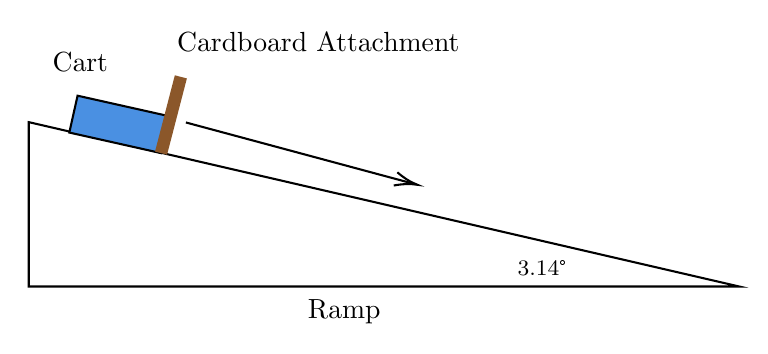
\begin{tikzpicture}[x=0.75pt,y=0.75pt,yscale=-1,xscale=1]
%uncomment if require: \path (0,300); %set diagram left start at 0, and has height of 300

%Shape: Right Triangle [id:dp18569224305294485] 
\draw   (3,189) -- (345.3,268.2) -- (3,268.2) -- cycle ;
%Shape: Rectangle [id:dp7438562411637597] 
\draw  [fill={rgb, 255:red, 74; green, 144; blue, 226 }  ,fill opacity=1 ] (26.54,176.27) -- (70.74,186.17) -- (66.76,203.93) -- (22.56,194.03) -- cycle ;
%Straight Lines [id:da735201395514776] 
\draw [color={rgb, 255:red, 139; green, 87; blue, 42 }  ,draw opacity=1 ][line width=4.5]    (76.3,167.2) -- (66.76,203.93) ;
%Straight Lines [id:da10025482914979356] 
\draw    (78.74,189.17) -- (188.37,218.68) ;
\draw [shift={(190.3,219.2)}, rotate = 195.06] [color={rgb, 255:red, 0; green, 0; blue, 0 }  ][line width=0.75]    (10.93,-3.29) .. controls (6.95,-1.4) and (3.31,-0.3) .. (0,0) .. controls (3.31,0.3) and (6.95,1.4) .. (10.93,3.29)   ;

% Text Node
\draw (237,254) node [anchor=north west][inner sep=0.75pt]   [align=left] {{\fontfamily{}\selectfont {\footnotesize 3.14°}}};
% Text Node
\draw (13,154) node [anchor=north west][inner sep=0.75pt]   [align=left] {{\fontfamily{}\selectfont Cart}};
% Text Node
\draw (73,144) node [anchor=north west][inner sep=0.75pt]   [align=left] {{\fontfamily{}\selectfont Cardboard Attachment}};
% Text Node
\draw (136,273) node [anchor=north west][inner sep=0.75pt]   [align=left] {{\fontfamily{}\selectfont Ramp}};


\end{tikzpicture}
\caption{General experimental setup with a \textit{Smart Cart} rolling down a ramp. Cross-sectional area of the cart is changed using a cardboard attachment.}
\end{figure}